\begin{marginfigure}
\begin{tikzpicture}
\node [name-dest] (box){%
    \begin{minipage}{0.80\textwidth}
     \begin{itemize}
    \item Rhys Tyers
    \item Clare Tan
    \end{itemize}
    \end{minipage}

};
\node[fancytitle, right=10pt] at (box.north west) {RCC Passage of the Year};
\end{tikzpicture}
\end{marginfigure}

\section{A Name Fit for the Lead}


\passage{Invictus} feels a long way from home. My pushing trip there with Tetley in 2012 were at the time the hardest thing I had physically done. I believe one of the trips I did was in excess of 22 hours. And now we were back to push further than the furthest there was. Clare and I, a crack team if ever there was one. 

\begin{marginsurvey}
\checkoddpage \ifoddpage \forcerectofloat \else \forceversofloat \fi
\centering
 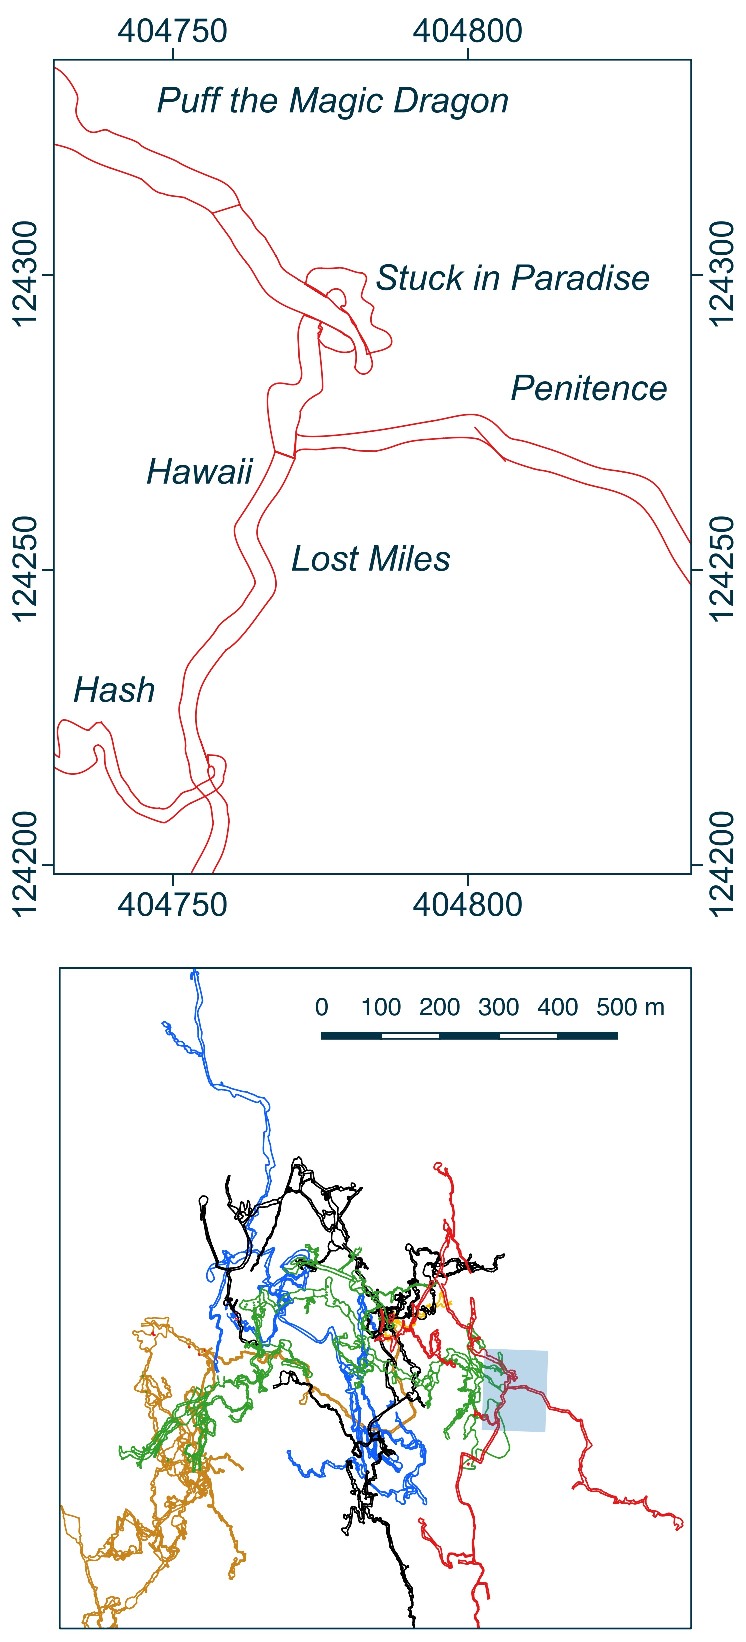
\includegraphics[width=\linewidth]{images/little_insets/hawaii_inset.pdf}
 \caption[Survey of Hash]{The \protect\passage{Hash} pushing front, Slovenian National Grid ESPG 3794}
 \label{Red Cow inset}
\end{marginsurvey}


Down the thick mud of \passage{Stuck in Paradise}, past the infested \passage{Hawaii} and into \passage{Penitence}. Half an hour or so of crawling on sharp pebbles. The sort that shatter as you place your weight on them. And then into the comparitive respite of \passage{Salvation}, where the floor is merely sand, but the ceiling no higher. Past the low junction, one side entirely full of sand. An easy dig were it 700m higher. Through the boulder choke that Tetley and I had cleared last year (and the one that had briefly entombed him). Onwards through the bizarre shattered chambers of \passage{Brave New World}, ignore the drippy inlet that almost certainly goes nowhere, squeeze past the ceiling slab collapse and pop out into \passage{Invictus}. Great piles of sand crowd the sides of the chamber.

At the end of the sandy passage we reached our goal, a pitch I had been forced to leave last year. Invictus intersects a shaft about halfway up. Maybe 15m to the bottom. A small stream falls down from the top. We place some bolts, chuck the rope down, promise to fix the rub point when the passage goes. We did not need to follow through on the promise. 

At the bottom, a typical flat, white, clean washed floor. The stream from above splattering and collecting gradually towards the far side of the chamber. There a passage leads off. We poked our heads in. A sump. Pretty and blue amongst the white rock, but its terminality spoiling its beauty. We searched for a while at the bottom, and up in Invictus for a way around but to no success. The aven is a potential lead, but the rock seemed chossy and loose. A difficult climb at best.

We named our lacklustre find \passage{RCC Passage of the Year} in honor of the lacklustre award we had recieved from the Union. We headed back out. 

Unquenched for exploration we elect to pop into \passage{Hash} on our way past. The tight, upwards spiralling, dry inlet off \passage{Minestrone} had been pushed by more people than it's nature deserved and had revealed the expected pittance of passage. Wiggling our way to the top, we found the small chamber in which Sam and Tetley had stopped. We push on, into more upwards tight crawl. After a short while we reach a dog leg in the passage that Clare did not want to attempt. Two things are known about Clare; she is small, and she is crazy. I suspect it would be deeply unwise for anyone larger or saner to attempt to push further. 

We surveyed out and climbed back towards X-Ray, arriving dissapointingly early. So early that we could not yet kick the sleepers out of bed. We are no inexperienced pair though, so we construct Camp Gamma Ray to ease our wait. A foil survival blanket thrown over a washing line forms a tent. A gas stove fills said tent with heat and carbon monoxide. So we pass the hazy hours till our designated slot in camp.

\name{Rhys Tyers}

\begin{figure*}[b!]
\begin{tikzpicture}
\node [name-dest] (box){%
    \begin{minipage}{0.95\textwidth}
    \begin{multicols}{2}
\paragraph{July 20$^{th}$} --- `Yesterday's trip to \passage{Minestrone} was a lot of fun. Looked at the little leads going off and Kate's climb. All became little squeezes with no draught. Except a climb (cairn at base of it) around PSS 21 and PSS 24, which leads to a downward sloping body sized tube which draughts. I went down it a good 5-10m but it seems to go on forever and felt too committing to do without help/rope. \passage{Hash} is a new lead found by Tim on the way back. Around 30-40m down Lost Miles from Hawaii is a climb up on the left hand side. PSS for \passage{Hash} is at start of climb. Left at draughting body sized crawl as we were short of time.' \name{Clare Tan}

\paragraph{July 22$^{nd}$} --- `Oh, also, we went and pushed \passage{Hash}, adding around 25 metres to what Tim \emph{et al.} had surveyed previously. Hash is fucking twatty and does continue beyond what we surveyed. Problem, only Tetley could fit through the squeezed just beyond our last survey leg. It was so close, just my shoulders are slightly too broad..with some tools we could've enlarged it but we would have had to gone back through to collect them. Beyond the squeeze, the passage continues upwards into a small chamber, 3m wide, 8m tall with a tight passage continuing off at the top. (all according to Tetley of course). Go push you narrow shouldered people.' \name{Sam Page}

\paragraph{August 1$^{st}$} ---`I am currently sat in a big silver bag in \passage{Friendship Gallery} with Clare. Today we pushed and killed \passage{Invictus}. It ends in a very tight rift with a puddle. The 20m of passage is named `\passage{RCC Passage of the Year}'. We also pushed \passage{Hash} to a tight chicane crawl thing that is is inadvisable for people bigger than Clare to go down. All in all got about 50m of passage. The silver bag, `Camp Gamma Ray' is very \sout{warm} grim.' \name{Rhys Tyers}
 \end{multicols}
    \end{minipage}

};
\node[fancytitle, right=10pt] at (box.north west) {The story of Hash --- the eventual death of a lead for the connoisseur};
\end{tikzpicture}
\end{figure*}